\chapter{End-to-End Application Methodology}

\section{Methodology Overview: How Lucid Builds an Investment Portfolio}
Building a sound investment portfolio requires combining human common sense with mathematical precision. In traditional wealth management, human financial advisors sit down with a client, evaluate their life goals, research companies in the stock market, and calculate how much money should be placed in each stock.

Lucid automates this entire process using an intelligent \textbf{16-step methodology}. The methodology bridges the gap between qualitative artificial intelligence and mathematical optimization. It ensures that every portfolio recommendation is personalized to the user, backed by verified exchange data, mathematically sound, and ready to be executed on real Indian stock exchanges.

The 16 steps are divided into four clear operational phases:
\begin{enumerate}
    \item \textbf{Phase I: Investor Profiling and Regulatory Suitability} (Steps 1--4): Lucid learns who the investor is, what they want to achieve, how much money they have, and how much financial risk they are comfortable taking.
    \item \textbf{Phase II: Market Research and Multi-Agent Analysis} (Steps 5--9): Lucid examines 2,639 listed Indian companies across the National Stock Exchange (NSE) and Bombay Stock Exchange (BSE), checks overall market health, evaluates company balance sheets, and uses a team of AI specialist agents to pick the most promising candidates.
    \item \textbf{Phase III: Mathematical Optimization and Whole-Share Calculations} (Steps 10--12): A mathematical solver calculates the safest and most profitable percentage weight for each stock. A rounding algorithm then converts these percentages into exact whole numbers of shares that can be purchased in the real world, accounting for government taxes and transaction fees.
    \item \textbf{Phase IV: Market-Hours Monitoring and Automatic Rebalancing} (Steps 13--16): Once the portfolio is created, a background monitoring daemon tracks live stock prices during market trading hours. If stock price fluctuations cause the portfolio to drift away from its planned balance, Lucid alerts the investor and provides a transparent before-and-after preview for rebalancing.
\end{enumerate}

Figure~\ref{fig:methodology_flow} illustrates how these 16 steps connect together in a seamless workflow:

\clearpage
\begin{figure}[p]
    \centering
    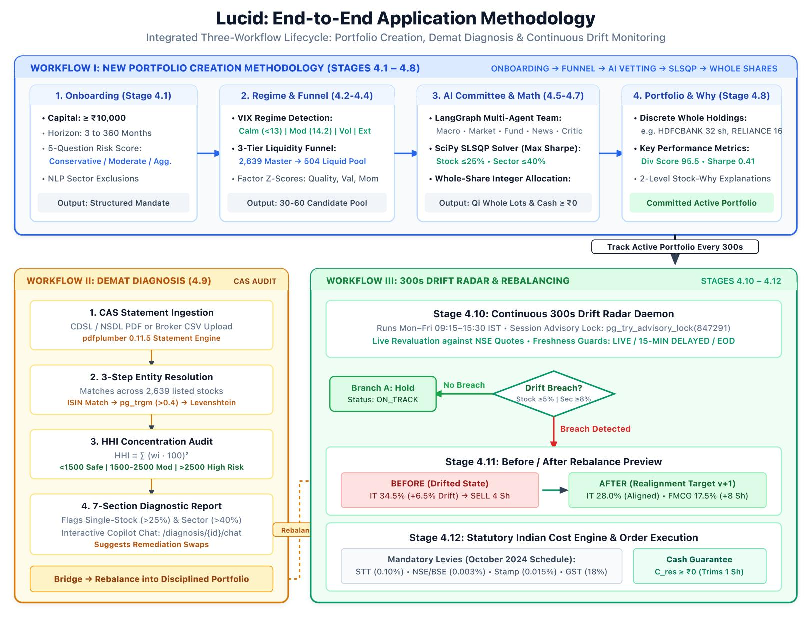
\includegraphics[width=0.92\textwidth, height=0.82\textheight, keepaspectratio]{METHODOLOGY_FLOW.pdf}
    \caption{Lucid Comprehensive 16-Step Investment Engineering Methodology}
    \label{fig:methodology_flow}
\end{figure}
\clearpage

\section{Phase I: Learning About the Investor and Establishing Rules}

\subsection{Step 1: Regulatory Suitability Questionnaire}
Before recommending any financial product, Indian regulations established by SEBI (the Securities and Exchange Board of India) require financial systems to understand an investor's background and risk appetite.

To achieve this, Lucid presents a 5-question suitability survey. Each question explores a crucial aspect of the investor's financial situation:
\begin{enumerate}
    \item \textbf{Market Knowledge and Experience}: Does the user understand how the stock market works, or are they a first-time investor?
    \item \textbf{Investment Time Horizon}: When will the investor need this money back? (Short-term: less than 1 year, Medium-term: 1 to 5 years, Long-term: more than 5 years).
    \item \textbf{Psychological Reaction to Losses}: If the stock market drops by 20\% in a single month, would the user panic and sell, stay calm, or see it as an opportunity to buy more shares at a discount?
    \item \textbf{Financial Goal Objective}: Is the primary goal protecting savings from inflation, achieving steady long-term growth, or pursuing aggressive wealth creation?
    \item \textbf{Income Stability}: Does the user have a predictable monthly salary or variable business income?
\end{enumerate}

Each answer choice carries a score between 1 and 4 points. The total suitability score $S$ is calculated by summing the weighted points:
\begin{equation}
S = \sum_{j=1}^{5} \omega_j \cdot x_j
\end{equation}
where $x_j$ is the answer score for question $j$ and $\omega_j$ is the question importance weight (defaulting to 1.0).

Based on the total score $S$ (ranging from 5 to 20), Lucid assigns the investor to one of three official \textbf{Risk Categories}:
\begin{equation}
\text{Risk Category} = 
\begin{cases} 
\textbf{Conservative} & \text{if } S \in [5, 9] \\ 
\textbf{Moderate} & \text{if } S \in [10, 15] \\ 
\textbf{Aggressive} & \text{if } S \in [16, 20] 
\end{cases}
\end{equation}

\noindent \textbf{Practical Example}: 
Suppose an investor scores a total of 12 points. Lucid classifies them as a \textbf{Moderate} investor. This classification tells the rest of the application to seek steady capital growth while avoiding excessively volatile or speculative stocks.

\subsection{Step 2: Natural Language Understanding and Custom Investor Rules}
Many retail investors find rigid multiple-choice forms intimidating. To make the process natural and accessible, Lucid allows investors to describe their investment goals in everyday language.

An investor can simply type:
\begin{quote}
\textit{``I have 2.5 lakhs to invest for my daughter's college education in 10 years. I want moderate risk, but please do not buy shares in any alcohol, tobacco, or defense companies.''}
\end{quote}

Lucid's language understanding module analyzes this sentence and extracts key facts:
\begin{itemize}
    \item \textbf{Investment Capital}: Converted into a numeric value: $\text{Rs.~}2,50,000$.
    \item \textbf{Investment Horizon}: Extracted as 10 years.
    \item \textbf{Financial Goal}: Tagged as an ``Education Goal.''
    \item \textbf{Risk Appetite}: Confirmed as ``Moderate.''
    \item \textbf{Excluded Sectors}: Mapped to industry exclusion rules: \texttt{FMCG\_TOBACCO}, \texttt{BEVERAGES\_ALCOHOL}, and \texttt{DEFENSE}.
\end{itemize}

\subsection{Step 3: Checking Overall Market Conditions (Market Regime)}
Stock markets do not behave the same way every day. Sometimes markets are calm and rising steadily; other times they are volatile, unpredictable, or falling rapidly during global crises.

To protect retail investors, Lucid checks the overall temperature of the Indian stock market before picking individual stocks:
\begin{enumerate}
    \item \textbf{Market Trend via Nifty 50 Moving Averages}:
    Lucid compares the current price of the Nifty 50 index ($P_{\text{Nifty}}$) against its 50-day Simple Moving Average ($\text{SMA}_{50}$) and 200-day Simple Moving Average ($\text{SMA}_{200}$):
    \begin{equation}
    \text{Market Trend} = 
    \begin{cases}
    \textbf{Bullish (Upward)} & \text{if } P_{\text{Nifty}} > \text{SMA}_{50} > \text{SMA}_{200} \\
    \textbf{Neutral (Sideways)} & \text{if } \text{SMA}_{50} \ge P_{\text{Nifty}} \ge \text{SMA}_{200} \\
    \textbf{Bearish (Downward)} & \text{if } P_{\text{Nifty}} < \text{SMA}_{200}
    \end{cases}
    \end{equation}
    \item \textbf{Market Volatility via India VIX}:
    The India Volatility Index (India VIX), often called the ``fear gauge,'' measures how much market fluctuation traders expect over the next 30 days:
    \begin{equation}
    \text{Volatility Tier} = 
    \begin{cases}
    \text{Low (Calm)} & \text{if } \text{VIX} < 13.0 \\
    \text{Normal (Stable)} & \text{if } 13.0 \le \text{VIX} \le 18.0 \\
    \text{Elevated (Nervous)} & \text{if } 18.0 < \text{VIX} \le 24.0 \\
    \text{Extreme (Panic)} & \text{if } \text{VIX} > 24.0
    \end{cases}
    \end{equation}
\end{enumerate}

When market volatility is high (VIX $> 18$), Lucid automatically becomes more cautious. It increases the risk-penalty factor ($\lambda$) in its calculations, favoring large, stable, dividend-paying companies over volatile smaller firms.

\subsection{Step 4: Ensuring Stock Liquidity and Safety}
A common trap for retail investors is buying shares in tiny or illiquid companies where very few shares are traded each day. In such stocks, an investor may find it impossible to sell their shares when they need their money back, or they may suffer large price losses due to a lack of buyers.

To protect users from illiquid stocks, Lucid maintains a synchronized master catalog of \textbf{2,639 listed Indian companies} and categorizes them into four institutional \textbf{Liquidity Tiers} based on their Average Daily Trading Volume (ADTV):

\begin{table}[H]
\centering
\caption{Lucid Stock Universe Liquidity Tier Classification}
\label{tab:liquidity_tiers}
\resizebox{\textwidth}{!}{%
\begin{tabular}{llccc}
\toprule
\textbf{Liquidity Tier} & \textbf{Market Segment / Description} & \textbf{Min Daily Shares} & \textbf{Min Daily Value (Rs.)} & \textbf{Eligible for Recommendation} \\
\midrule
\textbf{Tier 1: Ultra Liquid} & Nifty 50 and Nifty Next 50 blue-chip companies & $> 1,00,000$ & $> \text{Rs.~}1,00,00,000$ & \textbf{Yes (Top Priority)} \\
\textbf{Tier 2: Broad Liquid} & Nifty Midcap 150 established mid-sized companies & $> 50,000$ & $> \text{Rs.~}50,00,000$ & \textbf{Yes (High Priority)} \\
\textbf{Tier 3: Emerging Liquid} & Top half of Nifty Smallcap 250 growing companies & $> 10,000$ & $> \text{Rs.~}25,00,000$ & \textbf{Yes (Subject to Quality Filters)} \\
\textbf{Tier 4: Restricted} & Micro-caps, penny stocks, or suspended series & $< 10,000$ & $< \text{Rs.~}25,00,000$ & \textbf{No (Excluded to Protect Capital)} \\
\bottomrule
\end{tabular}%
}
\end{table}

All active equities across the 2,639 listed exchange securities are evaluated dynamically. Only actively traded shares meeting institutional liquidity standards are recommended for new portfolios, while Tier 4 stocks remain searchable so investors can analyze historical holdings imported from their existing Demat statements.

\section{Phase II: Stock Research and Multi-Agent Evaluation}

\subsection{Step 5: Examining Company Financial Fundamentals}
Just as a doctor examines vital signs before certifying a person healthy, Lucid examines six core financial metrics for each eligible company:
\begin{enumerate}
    \item \textbf{Return on Equity (ROE)}: Measures how efficiently a company generates profits from the money shareholders have invested:
    \begin{equation}
    \text{ROE} = \frac{\text{Annual Net Profit}}{\text{Total Shareholders' Equity}} \times 100\%
    \end{equation}
    Lucid prefers companies with an $\text{ROE} \ge 15\%$, showing strong profitability.
    \item \textbf{Price-to-Earnings (P/E) Ratio}: Compares the company's stock price to its annual earnings per share. This shows whether a stock is cheap or expensive relative to industry peers.
    \item \textbf{Debt-to-Equity Ratio (D/E)}: Compares the company's total borrowings to its net worth. Lucid strictly requires $\text{D/E} \le 1.5$ for non-banking companies, ensuring the business is not at risk of bankruptcy from heavy debt burdens.
    \item \textbf{Operating Cash Flow}: Verifies that reported accounting profits represent real cash flowing into bank accounts rather than uncollected promises.
    \item \textbf{Historical Price Volatility ($\sigma_i$)}: Measures how widely the stock's price has fluctuated over the past 252 trading sessions (one full year).
    \item \textbf{Market Beta ($\beta_i$)}: Measures how sensitive the stock is to broad market movements. A stock with $\beta = 1.0$ moves in sync with the Nifty 50; a stock with $\beta = 1.5$ is 50\% more volatile than the market; and a stock with $\beta = 0.7$ is more defensive and stable.
\end{enumerate}

\subsection{Step 6 to Step 9: The Multi-Agent Research Team in Action}
Once quantitative screening narrows the stock universe to roughly 50 promising companies, Lucid's team of 13 AI agents conducts in-depth qualitative evaluation:
\begin{itemize}
    \item \textbf{Macro Analyst Agent}: Reviews current Reserve Bank of India (RBI) interest rates and inflation figures to identify which industries will benefit from the current economic climate.
    \item \textbf{Sector Specialist Agents}: Examine company competitive advantages (known as economic moats), such as strong brand names, technological leadership, or distribution networks.
    \item \textbf{News and Sentiment Agent}: Reads recent news articles to identify any legal disputes, management scandals, or regulatory investigations that might endanger the company.
    \item \textbf{Adversarial Critic Agent}: Acts as a professional skeptic. The Critic specifically searches for weaknesses or warning signs in the candidate companies, challenging overly optimistic opinions and eliminating candidates with hidden risks.
\end{itemize}

At the conclusion of this process, the agents produce a finalized shortlist of 15 to 25 high-quality companies, along with conviction ratings and plain-English reasons for their selection.

\section{Phase III: Mathematical Optimization and Real-World Execution}

\subsection{Step 10: Modern Portfolio Optimization (SciPy SLSQP)}
A key design principle of Lucid is that \textbf{AI agents are never allowed to calculate stock numbers, percentages, or money allocations}. When artificial intelligence models attempt numerical calculations, they can produce mathematical errors or invent numbers out of thin air.

Instead, Lucid passes the candidate shortlist to a proven, deterministic mathematical engine that uses the \textbf{Sequential Least Squares Programming (SLSQP)} solver from the scientific library \texttt{scipy.optimize}.

\noindent \textbf{The Optimization Goal}:
Depending on the investor's risk profile, the solver maximizes the \textbf{Sharpe Ratio} (the amount of investment return earned per unit of risk taken):
\begin{equation}
\max_{\mathbf{w}} \text{Sharpe Ratio} = \frac{\mathbf{w}^T \boldsymbol{\mu} - R_f}{\sqrt{\mathbf{w}^T \mathbf{\Sigma} \mathbf{w}}}
\end{equation}
where:
\begin{itemize}
    \item $\mathbf{w} = [w_1, w_2, \dots, w_K]^T$ is the vector of percentage weights allocated to each stock.
    \item $\boldsymbol{\mu} = [\mu_1, \mu_2, \dots, \mu_K]^T$ is the expected annual return for each stock based on historical performance.
    \item $R_f$ is the risk-free return rate in India (the interest rate paid by safe Indian government treasury bills, set at 7.0\% per year).
    \item $\mathbf{\Sigma}$ is the covariance matrix measuring how the prices of the different stocks move together. If two stocks move in opposite directions, combining them lowers total portfolio risk.
\end{itemize}

\noindent \textbf{Strict Financial Rules (Constraints)}:
The solver must satisfy three mandatory safety rules:
\begin{enumerate}
    \item \textbf{100\% Capital Allocation}: The weights of all stocks must add up to exactly 100\%:
    \begin{equation}
    \sum_{i=1}^{K} w_i = 1.0 \quad (100\%)
    \end{equation}
    \item \textbf{No Borrowing or Short Selling}: Every stock weight must be non-negative:
    \begin{equation}
    w_i \ge 0.0 \quad \text{for all stocks } i
    \end{equation}
    \item \textbf{Single-Stock Cap (Maximum 25\%)}: To prevent excessive exposure to any single company, no stock may exceed 25\% of the portfolio:
    \begin{equation}
    w_i \le 0.25 \quad (25\%)
    \end{equation}
    \item \textbf{Sector Diversification Cap (Maximum 40\%)}: To protect the investor against an industry downturn, all stocks belonging to the same sector (such as Information Technology or Banking) combined must not exceed 40\%:
    \begin{equation}
    \sum_{i \in \text{Sector}_m} w_i \le 0.40 \quad (40\%)
    \end{equation}
\end{enumerate}

\subsection{Step 11: Converting Weights into Whole Shares}
Under Indian stock market regulations, shares must be purchased as whole units. An investor cannot buy 3.42 shares of a company; they can only buy 3 shares or 4 shares.

Because the optimizer calculates continuous weights (such as 14.32\%), Lucid translates these percentages into whole share counts without exceeding available capital $C$.

\noindent \textbf{Stage 1: Floor Rounding}:
For each stock $i$ with calculated weight $w_i^*$ and current price $P_i$, the initial whole-share quantity $q_i$ is determined by rounding down:
\begin{equation}
q_i = \left\lfloor \frac{C \cdot w_i^*}{P_i} \right\rfloor
\end{equation}
The total money allocated across all shares is:
\begin{equation}
C_{\text{alloc}} = \sum_{i=1}^{K} q_i \cdot P_i
\end{equation}
The leftover unallocated cash $C_{\text{residual}}$ is:
\begin{equation}
C_{\text{residual}} = C - C_{\text{alloc}} \ge 0
\end{equation}

\noindent \textbf{Stage 2: Cash Remainder Allocation}:
If leftover cash remains ($C_{\text{residual}} > 0$), Lucid checks whether one additional share of the highest-conviction stocks can be bought without violating the 25\% single-stock limit:
\begin{equation}
(q_j + 1) \cdot P_j \le C_{\text{alloc}} + C_{\text{residual}} \quad \text{and} \quad \frac{(q_j + 1) \cdot P_j}{C} \le 0.25
\end{equation}
If the share fits within the budget, it is added. Any tiny remainder that cannot purchase a full share is preserved in the investor's cash reserve balance. Not a single rupee is lost or unaccounted for.

\noindent \textbf{Simple Numerical Example}:
Suppose an investor has $C = \text{Rs.~}50,000$, and the solver allocates a 15\% weight ($w_1^* = 0.15$, or Rs.~7,500) to Infosys, trading at $P_1 = \text{Rs.~}1,800$ per share:
\begin{equation}
q_1 = \left\lfloor \frac{7500}{1800} \right\rfloor = \lfloor 4.167 \rfloor = 4 \text{ whole shares}
\end{equation}
The 4 shares cost $4 \times 1800 = \text{Rs.~}7,200$, leaving Rs.~300 in the cash reserve pool for other purchases.

\subsection{Step 12: Statutory Indian Tax and Transaction Fee Modeling}
When an investor buys or sells shares on the Indian stock market, mandatory government taxes and exchange fees are charged. Lucid calculates these fees transparently so the user sees the exact total cost before executing any trade.

Table~\ref{tab:transaction_costs} lists the official fee rates applied by Lucid:

\begin{table}[H]
\centering
\caption{Statutory Indian Equity Delivery Transaction Fee Schedule}
\label{tab:transaction_costs}
\resizebox{\textwidth}{!}{%
\begin{tabular}{llcc}
\toprule
\textbf{Fee Component} & \textbf{Authority / Legal Basis} & \textbf{Buy Rate} & \textbf{Sell Rate} \\
\midrule
\textbf{Securities Transaction Tax (STT)} & Department of Revenue, Govt. of India & 0.1000\% & 0.1000\% \\
\textbf{Exchange Turnover Charge} & NSE / BSE & 0.00325\% & 0.00325\% \\
\textbf{SEBI Turnover Fee} & Securities and Exchange Board of India & 0.0001\% (Rs.~10 per Cr) & 0.0001\% (Rs.~10 per Cr) \\
\textbf{Stamp Duty} & Indian Stamp Act (Govt. of India) & 0.0150\% & 0.0000\% \\
\textbf{Brokerage (Discount Broker Profile)} & Broker Platform (Zerodha / Groww profile) & Rs.~0.00 & Rs.~0.00 \\
\textbf{Goods and Services Tax (GST)} & Ministry of Finance, Govt. of India & 18\% on (Brokerage + Txn + SEBI) & 18\% on (Brokerage + Txn + SEBI) \\
\bottomrule
\end{tabular}%
}
\end{table}

\noindent \textbf{Numerical Example}:
For a purchase of $\text{Rs.~}1,00,000$ worth of delivery equity shares:
\begin{itemize}
    \item $\text{STT} = 0.10\% \times 1,00,000 = \text{Rs.~}100.00$
    \item $\text{Stamp Duty} = 0.015\% \times 1,00,000 = \text{Rs.~}15.00$
    \item $\text{Exchange Fee} = 0.00325\% \times 1,00,000 = \text{Rs.~}3.25$
    \item $\text{SEBI Fee} = 0.0001\% \times 1,00,000 = \text{Rs.~}0.10$
    \item $\text{GST} = 18\% \times (3.25 + 0.10) = \text{Rs.~}0.60$
    \item \textbf{Total Statutory Fees}:
    \[
    \text{Total Friction} = 100.00 + 15.00 + 3.25 + 0.10 + 0.60 = \text{Rs.~}118.95
    \]
    This equals only about 0.12\% of the total trade value.
\end{itemize}

\section{Phase IV: Market Monitoring, Diagnosis, and Fiduciary Explanations}

\subsection{Step 13: Demat Portfolio (CAS) Diagnosis}
Many investors already hold existing stocks purchased across multiple broker platforms (such as Zerodha, Groww, or Angel One). To give these investors clarity on their current investments, Lucid includes an automated Demat statement diagnostic tool.

The user simply uploads their official monthly Consolidated Account Statement (CAS PDF) provided by CDSL or NSDL. Lucid parses the PDF, extracts every stock held, and evaluates:
\begin{enumerate}
    \item \textbf{Herfindahl-Hirschman Index (HHI)}:
    Measures whether the investor's money is concentrated dangerously in too few companies:
    \begin{equation}
    \text{HHI} = \sum_{i=1}^{N} (s_i \times 100)^2
    \end{equation}
    where $s_i$ is the share of total portfolio wealth in stock $i$. An $\text{HHI} > 2500$ indicates severe concentration risk (for example, having 60\% of wealth in a single stock).
    \item \textbf{Overlapping Holdings and Sector Skews}: Identifies whether the user is accidentally overexposed to a single industry (such as holding six different banking stocks that make up 55\% of their money).
    \item \textbf{Actionable Health Ratings}: Marks each position with a clear recommendation: \textbf{Keep (Hold)}, \textbf{Add (Buy)}, \textbf{Trim (Sell)}, or \textbf{No Action Needed}.
\end{enumerate}

\subsection{Step 14: Continuous Background Monitoring and Drift Radar}
Once a portfolio is active, its stock weights do not stay constant. If one stock doubles in price while another stays flat, the first stock becomes a much larger percentage of the portfolio than originally intended. This unintended shift is called \textbf{portfolio drift}.

Lucid's background monitoring service evaluates all active portfolios every 300 seconds (5 minutes) during official Indian exchange trading hours (Monday through Friday, 09:15 to 15:30 IST).

The drift for each stock $i$ at time $t$ is calculated as the difference between its current actual weight $w_i(t)$ and its planned target weight $w_{i,\text{target}}$:
\begin{equation}
\text{Drift}_i(t) = \left| \frac{q_i \cdot P_i(t)}{\sum_{j=1}^{K} q_j \cdot P_j(t) + C_{\text{cash}}} - w_{i,\text{target}} \right|
\end{equation}

If any single stock's weight moves away from its target by 5\% or more, or if an entire industry sector moves by 8\% or more:
\begin{equation}
\max_{i} \text{Drift}_i(t) \ge 0.05 \quad (5\%) \quad \lor \quad \max_{m} \text{SectorDrift}_m(t) \ge 0.08 \quad (8\%)
\end{equation}
Lucid automatically triggers a \textbf{Rebalance Alert}.

\subsection{Step 15: Rebalance Impact Preview}
When a rebalance alert is triggered, Lucid does not execute trades silently or automatically. Instead, it prepares a transparent \textbf{Rebalance Impact Preview} for the investor:
\begin{itemize}
    \item Shows the exact proposed trades (for example: ``Sell 5 shares of Stock A, Buy 3 shares of Stock B'').
    \item Displays the portfolio balance before and after the proposed adjustment.
    \item Calculates the statutory taxes and transaction fees that will be charged.
    \item Guarantees that the cash required for new purchases does not exceed the proceeds from sales plus available cash reserves.
\end{itemize}
The investor remains in complete control and can inspect the exact impact before approving the rebalancing action.

\subsection{Step 16: Dual-Level Fiduciary ``Stock-Why'' Explanations}
Most robo-advisors show users a pie chart with stock names, giving no explanation as to why those particular companies were selected. This lack of transparency causes anxiety for retail investors.

To eliminate this ``black box,'' Lucid provides a \textbf{dual-level explanation} for every recommended stock:
\begin{enumerate}
    \item \textbf{Retail Narrative Tier (For Everyday Investors)}: A conversational, easy-to-read explanation explaining the company's business model, competitive advantages, and why it fits the user's specific investment goal.
    \item \textbf{Quantitative Metric Tier (For Serious Investors)}: A verifiable financial scorecard showing the company's Return on Equity (ROE), P/E ratio, Debt-to-Equity ratio, 1-year historical return, market beta, and its mathematical contribution to portfolio diversification.
\end{enumerate}

This dual-tier approach ensures that both novice investors and experienced traders have complete confidence and transparency in every investment recommendation.
